% Communication job: show one input processed in parallel and fused once.
% Primary grammar: fan-out/fan-in parallel pipeline.
% Target geometry: single-column figure, natural width approximately 8.5 cm or less.
% Semantic status: schematic.
% Compile with: pdflatex parallel-pipeline.tex
\documentclass[tikz,border=2mm,10pt]{standalone}

\usetikzlibrary{arrows.meta,positioning,calc}

\definecolor{figdark}{gray}{0.25}
\definecolor{figlight}{gray}{0.85}

\tikzset{
  terminal/.style={
    rectangle, draw=figdark, fill=white,
    minimum width=1.05cm, minimum height=0.65cm,
    align=center, inner sep=3pt
  },
  block/.style={
    rectangle, draw=figdark, fill=figlight,
    minimum width=1.45cm, minimum height=0.70cm,
    align=center, inner sep=3pt
  },
  arrow/.style={->, >={Stealth[length=1.8mm]}, thick, draw=figdark},
  wire/.style={thick, draw=figdark}
}

\begin{document}
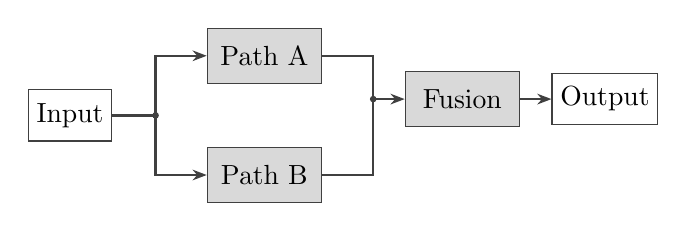
\begin{tikzpicture}[node distance=0.60cm and 0.80cm]
  \node[terminal] (input) {Input};
  \coordinate[right=0.55cm of input] (split);
  \node[block, above right=0.40cm and 0.65cm of split] (patha) {Path A};
  \node[block, below right=0.40cm and 0.65cm of split] (pathb) {Path B};
  \coordinate[right=0.65cm of patha.east, yshift=-0.55cm] (merge);
  \node[block, right=0.40cm of merge] (fusion) {Fusion};
  \node[terminal, right=0.40cm of fusion] (output) {Output};

  \draw[wire] (input.east) -- (split);
  \fill[figdark] (split) circle (1.2pt);
  \draw[arrow] (split) |- (patha.west);
  \draw[arrow] (split) |- (pathb.west);

  \draw[wire] (patha.east) -| (merge);
  \draw[wire] (pathb.east) -| (merge);
  \fill[figdark] (merge) circle (1.2pt);
  \draw[arrow] (merge) -- (fusion.west);
  \draw[arrow] (fusion) -- (output);
\end{tikzpicture}
\end{document}
